\documentclass[oneside,11pt,openright]{report}
\usepackage[latin1]{inputenc}
\usepackage{listings}
\usepackage[american]{babel}
\usepackage{a4}
\usepackage{latexsym}
\usepackage{amssymb}
\usepackage{amsmath}
\usepackage{amsthm}
\usepackage{epsfig}
\usepackage[T1]{fontenc}
\usepackage{lmodern}
\usepackage[labeled]{multibib}
\usepackage{color}
\usepackage{datetime}
\usepackage{epstopdf} 
\usepackage{graphicx}
\usepackage{pgfplots}
\usepackage[format=hang]{caption}
\usepackage{float}

\usepackage{pgf,tikz}
\usepackage{comment}
\usetikzlibrary{arrows,automata}
\usetikzlibrary{backgrounds,fit}
\usetikzlibrary{shapes,patterns}
\usetikzlibrary{calc,chains,positioning}

\renewcommand*\ttdefault{txtt}
\newcommand{\BigO}[1]{\ensuremath{\operatorname{O}\left(#1\right)}}
\newcommand{\BigT}[1]{\ensuremath{\Theta\left(#1\right)}}
\newcommand{\specialcell}[2][c]{%
  \begin{tabular}[#1]{@{}c@{}}#2\end{tabular}}
% see http://imf.au.dk/system/latex/bog/

\newcommand{\adjustimg}{% Horizontal adjustment of image
  \ifodd\value{page}\hspace*{\dimexpr\evensidemargin-\oddsidemargin}\else\hspace*{-\dimexpr\evensidemargin-\oddsidemargin}\fi%
}
\newcommand{\centerimg}[2][width=\textwidth]{% Center an image
  \makebox[\textwidth]{\adjustimg\inputgraphics[#1]{#2}}%
}
\newcommand{\NULL}{\textbf{null}}
\newcommand{\cons}{\textbf{cons}}
\newcommand{\cdr}{\textbf{cdr}}

\newcommand{\MakeList}{\textsc{makeList}(x)}
\newcommand{\Push}{\textsc{push}(x,L)}
\newcommand{\Pop}{\textsc{pop}(L)}
\newcommand{\Lookup}{\textsc{Lookup}(d)}
\newcommand{\Inject}{\textsc{inject}(x,L)}
\newcommand{\Eject}{\textsc{eject}(L)}
\newcommand{\Catenate}{\textsc{catenate}(K,L)}

\newtheorem{prop}{Property}
\newtheorem{theorem}{Theorem}

\begin{document}

%%%%%%%%%%%%%%%%%%%%%%%%%%%%%%%%%%%%%%%%%%%%%%%%%%%%%%%%%%%%%%%%%%%%%%%

\pagestyle{empty} 
\pagenumbering{roman} 
\vspace*{\fill}\noindent{\rule{\linewidth}{1mm}\\[4ex]
{\Huge\sf Functional Queues}\\[4ex]
{\huge\sf Kristoffer Just Andersen, 20051234\\[2ex]
\huge\sf Troels Leth Jensen, 20051234 \\[2ex]
\huge\sf Morten Krogh-Jespersen, 20022362}\\[2ex]
\noindent\rule{\linewidth}{1mm}\\[4ex]
\noindent{\Large\sf Project 3, Advanced Data Structures 2013, Computer Science\\[1ex] 
\monthname\ \the\year  \\[1ex] Advisor: Gerth St�lting Brodal\\[15ex]}\\[\fill]}
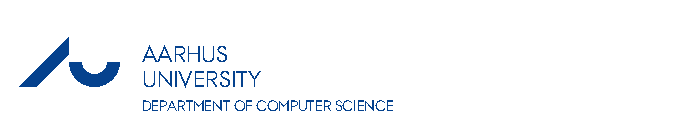
\epsfig{file=logo.eps}\clearpage

%%%%%%%%%%%%%%%%%%%%%%%%%%%%%%%%%%%%%%%%%%%%%%%%%%%%%%%%%%%%%%%%%%%%%%%

\tableofcontents
\pagenumbering{arabic}
\setcounter{secnumdepth}{2}

%%%%%%%%%%%%%%%%%%%%%%%%%%%%%%%%%%%%%%%%%%%%%%%%%%%%%%%%%%%%%%%%%%%%%%%

\chapter{Introduction}

needs content

\section{Terminology}

Purely functional

Strict evelaution

Lazy evaluation

Memoization

\chapter{A purely functional list as a queue}

\begin{center}
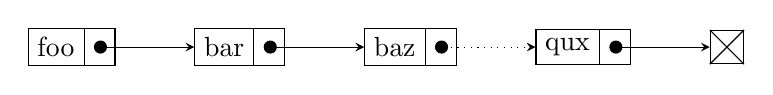
\begin{tikzpicture}
    [list/.style={rectangle split, rectangle split parts=2,
    draw, rectangle split horizontal}, >=stealth, start chain,
    pointer/.style = {font=\tt, anchor=base, inner sep=2pt}]

  \node[list,on chain] (A) {foo};
  \node[list,on chain] (B) {bar};
  \node[list,on chain] (C) {baz};
  \node[list,on chain] (D) {qux};
  \node[on chain,draw,inner sep=6pt] (E) {};

  \draw (E.north east) -- (E.south west);
  \draw (E.north west) -- (E.south east);
  \draw[*->] let \p1 = (A.two), \p2 = (A.center) in (\x1,\y2) -- (B);
  \draw[*->] let \p1 = (B.two), \p2 = (B.center) in (\x1,\y2) -- (C);
  \draw[dotted,*->] let \p1 = (C.two), \p2 = (C.center) in (\x1,\y2) -- (D);
  \draw[*->] let \p1 = (D.two), \p2 = (D.center) in (\x1,\y2) -- (E);

\end{tikzpicture}
\captionof{figure}{A purely functional list}
\label{fig:list_figure}
\end{center}

Figure \ref{fig:list_figure} shows a graphically representation of a functional list where elements can be inserted at the front by means of $\cons$ and the list can be traversed by following the arrows which corresponds to the $\cdr$ operation. The list can be constructed in constant time by a special termination construction (inductive base case) being the empty list.

Elements can be inserted and removed from the front in constant time, but all other operations require traversing the entire list. Below is all operations with the corresponding time-complexities shown:

\begin{center}
  \begin{tabular}{ l | c | c}
    Operation & List \\ \hline
    \MakeList & $\BigO{1}$ \\ 
    \Push & $\BigO{1}$ \\ 
    \Pop & $\BigO{1}$ \\ 
    \Inject & $\BigO{n}$ \\ 
    \Eject & $\BigO{n}$ \\ 
    \Catenate & $\BigO{|K|}$ \\ 
  \end{tabular}
\end{center}

\chapter{Queue by a pair of lists}

A simple observation to make is that if we reverse the list of section 2, $\Inject$ and $\Eject$ will be at the front of the list and will therefore take $\BigO{1}$ time, however, $\Push$ and $\Pop$ will take $\BigO{n}$ time. A trick is therefore to maintain a pair of lists such that $\Push$, $\Pop$, $\Inject$ and $\Eject$ for the most part perform in constant time.

\begin{center}
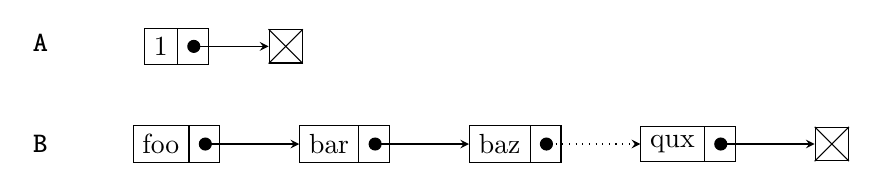
\begin{tikzpicture}
    [list/.style={rectangle split, rectangle split parts=2,
    draw, rectangle split horizontal}, >=stealth, start chain,
    desc/.style = {font=\tt, anchor=base, inner sep=2pt}]

  \node[desc, on chain] (list_b) {B};
  \node[list,on chain] (A) {foo};
  \node[list,on chain] (B) {bar};
  \node[list,on chain] (C) {baz};
  \node[list,on chain] (D) {qux};
  \node[on chain,draw,inner sep=6pt] (E) {};

  \node[desc, above=6ex of list_b] (list_a) {A};
  \node[list, above=5ex of A] (F) {1};
  \node[right=5ex of F,draw,inner sep=6pt] (G) {};

  \draw (G.north east) -- (G.south west);
  \draw (G.north west) -- (G.south east);
  \draw[*->] let \p1 = (F.two), \p2 = (F.center) in (\x1,\y2) -- (G);

  \draw (E.north east) -- (E.south west);
  \draw (E.north west) -- (E.south east);
  \draw[*->] let \p1 = (A.two), \p2 = (A.center) in (\x1,\y2) -- (B);
  \draw[*->] let \p1 = (B.two), \p2 = (B.center) in (\x1,\y2) -- (C);
  \draw[dotted,*->] let \p1 = (C.two), \p2 = (C.center) in (\x1,\y2) -- (D);
  \draw[*->] let \p1 = (D.two), \p2 = (D.center) in (\x1,\y2) -- (E);

\end{tikzpicture}
\captionof{figure}{Maintaining two lists - reverse on next pop}
\label{fig:two_lists_before_reverse}
\end{center}

When enqueueing nodes are pushed to the front of the list B and when elements are removed they are taken from the front of the list A which both performs in constant time. The only problem is what to do if A consists of only the empty list.

Figure ~\ref{fig:two_lists_before_reverse} shows a configuration of the queue where a pop will result in A becoming the empty list. Subsequent pops should remove from the end of B but that would take $\BigO{n}$ for every operation. It therefore makes 
more sense to reverse the list once and place instead of A.

POTENTIAL

Reversing the list can be done in $\BigO{n}$ where $n$ is the size of the list B. The length of B is the number of enqueues since the last reversal or construction of the list. By amortizing the cost of reversal over said enqueue-operations will result in all operations, except catenation, having $\BigO{1}$ time complexities:

\begin{center}
  \begin{tabular}{ l | c | c}
    Operation & List & Two lists (amortized) \\ \hline
    \MakeList & $\BigO{1}$ & $\BigO{1}$ \\ 
    \Push & $\BigO{1}$ & $\BigO{1}$ \\ 
    \Pop & $\BigO{1}$ & $\BigO{1}$ \\ 
    \Inject & $\BigO{n}$ & $\BigO{1}$ \\ 
    \Eject & $\BigO{n}$ & $\BigO{1}$ \\ 
    \Catenate & $\BigO{|K|}$ & $\BigO{min(|K|,|L|)}$ \\ 
  \end{tabular}
\end{center}

Catenation can be done in $\BigO{min(|K|,|L|)}$ although that requires maintaining the length of each queue. If $K$ has the fewest elements. then all elements from $K_B$ can be pushed to $L_A$ in constant time for each node, hereafter $K_B$ can be reversed and then pushed to $L_A$ which in total takes linear time in the size of $K$.
If $|L|$ is smaller then $L_A$ can be added $K_B$ as before and the result can be added as $\cdr$ to the list of $L_B$ which in all takes linear time in the size of $L$. WHAT ABOUT POTENTIAL?

\section{Converting to strict in Haskell}

Skriv at denne kan laves strict i haskell ved at anvende !

\chapter{Pair of lists with lazy evaluation}

We were asked to implement a queue with lazy evaluation having amortized constant time for all operations except concatination. As so many implementations we have two lists; one representing the front and another representing the tail. At specific points we will rotate the elements from the tail onto the head by reversing the tail list and appending it. In Haskell the append and the reverse function is lazy giving us the desired evalution strategy.

The trick with two lists has already been used in the previous chapter but we will use another trigger for the lazy implementation. We rotate whenever the length of the tail list is one greater than the length of the front list.

\section{Analyzing lazy evaluations}


\section{Completing the analysis of the lazy queue}

To perform the amortized analysis we will again use the potential function, however, the potential function is no longer equivalent to the elements in the tail. In fact, it is  

As always, it should be the case that we add potential on inserts and release potential when deleting. We therefore define the potential to be:
\begin{align*}
  \Phi(Q) = tail(Q) + notreversed(Q)
\end{align*}

Appending the reversed elements from the tail onto the head makes no change to the potential. Potential is released when a lazy list is demanded. Since any lazy list demanded will origin from the tail, the number of operations is completely specified by the amount of inserts and thus the release of potential pays for the reverting the list.

The above analysis assumes that when a demand for the first element of a lazy list not yet reversed, the list is reversed and all subsequent calls to the list will work in constant time. The latter part assumes therefore that lazy lists are memoized. We can now present the time complexities for the lazy algorithm:

\begin{center}
  \begin{tabular}{ l | c | c | c }
    Operation & List & \specialcell{Two lists\\(amortized)} & \specialcell{Lazy\\(amortized)} \\ \hline
    \MakeList & $\BigO{1}$ & $\BigO{1}$ & $\BigO{1}$ \\ 
    \Push & $\BigO{1}$ & $\BigO{1}$ & $\BigO{1}$ \\ 
    \Pop & $\BigO{1}$ & $\BigO{1}$ & $\BigO{1}$ \\ 
    \Inject & $\BigO{n}$ & $\BigO{1}$ & $\BigO{1}$ \\ 
    \Eject & $\BigO{n}$ & $\BigO{1}$ & $\BigO{1}$ \\ 
    \Catenate & $\BigO{|K|}$ & $\BigO{min(|K|,|L|)}$ & $\BigO{1}$ \\ 
  \end{tabular}
\end{center}

Catenating two queues can be done in constant time by appending the head of $L$ and the reversed tail of $L$ onto the head of $K$ because append and reverse are lazy thus the functions returns immediately. We assume that all unreleased potential of $L$ can be transferred to $K$.

\chapter{$\BigO{1}$ lists with worst case $\BigO{1}$ enqueue and dequeue with strict evaluation}

All of the queues described above have worst case running times $\BigO{n}$ which is unacceptable in some situations thus there exist a need for real times queues where all operations have worst case running times $\BigO{1}$. We have chosen to implement the Hood-Melville real time queue[REF].

There is a few key insights to this algorithm. First, reversing a list incrementally can be done by having two lists and transferring elements from one to the other. Second, one can incrementally append two lists by applying the trick. If one will would like to append two lists $xs$ and $ys$, one can reverse $xs$ to $xs'$ and then reverse $xs'$ onto $ys$. Additionally, one can reverse $xs$ on to the reverse of $ys$ by reversing $xs$ and $ys$ in parallel and then continue as before.

Initially, the queue will have two lists forming the head $H$ and tail $T$ and two integers describing the length of each. When we decide to rotate we use the observation above and do the following:

\begin{enumerate}
\item Reverse $T$ forming the tail of the new resulting head $H'$
\item Reverse $H$ into $H_R$
\item Reverse $H_R$ onto $H'$
\end{enumerate}

One should be able to convince himself (or herself) that queue order is preserved after the third step. However, the queue will not remain constant when performing the rotation (which is a weird phrase in [REF] since the incremental rotation only occurs when changes occur), but basically, it means that we have to maintain the state of the current rotation and provide the user the ability to still make alterations to the queue. 

Allowing the user to enqueue elements is easily done by just having a new tail list. Dequeueing is bit harder because we are currently reversing the $H$ into $H_R$. The answer is two have two lists; one being the a working copy of the old list and one being the list we are reversing. This again introduce some maintenance because removing an element from the working copy somehow has to be synchronized with the list we are reversing. To correct this, we use a counter that describe how many valid elements to be copied from $H_R$. A total of six lists is therefore necessary for this data structure.

The recopying (or rotation) should be completed before the first element is needed. We will rotate elements when the tail list becomes one longer than the head list, therefore, rotating elements will take $2m + 1$ operations where $m$ is the number of elements in head and tail. Therefore $2m + 1$ incremental operations must be performed in at most $m$ queue operations. By performing the two first rotation steps starting the rotation process and hereafter perform two incremental steps for each queue operation. In total, this gives $2(m+1) = 2m + 2$ steps, which is greater than $2m + 1$. We therefore perform constant work for every queue operation sans catenation:

\begin{center}
  \begin{tabular}{ l | c | c | c | c}
    Operation & List & \specialcell{Two lists\\(amortized)} & \specialcell{Lazy\\(amortized)} & Hood-Melville \\ \hline
    \MakeList & $\BigO{1}$ & $\BigO{1}$ & $\BigO{1}$ & $\BigT{1}$ \\ 
    \Push & $\BigO{1}$ & $\BigO{1}$ & $\BigO{1}$ & $\BigT{1}$ \\ 
    \Pop & $\BigO{1}$ & $\BigO{1}$ & $\BigO{1}$ & $\BigT{1}$ \\ 
    \Inject & $\BigO{n}$ & $\BigO{1}$ & $\BigO{1}$ & $\BigT{1}$ \\ 
    \Eject & $\BigO{n}$ & $\BigO{1}$ & $\BigO{1}$ & $\BigT{1}$ \\ 
    \Catenate & $\BigO{|K|}$ & $\BigO{min(|K|,|L|)}$ & $\BigO{1}$ & \\ 
  \end{tabular}
\end{center}

\chapter{Testing and correctness}

\chapter{Time measurements}

We have a total of five queues - three stricts and two lazy. We are asked to design experiments where a queue is only used once and also where the queue can be arbitrarily used. In this chapter we explain how we ensure lazy constructs are evaluated when testing, we describe the different tests that we apply to the queues and we discuss the results of said tests. 

\section{Making sure that lazy evaluations gets evaluated}

\section{One punch tests}

In this chapter we define only the tests that uses queues ..

We have designed two tests that enable us to directly measure tiem of insertions and deletions. However, a queue is useful for more things than theoretic time analysis so we are also using the queue to do Breadth-First search in graphs. 

\subsection{Time of insert}

This tests is analogue to the insert test we performed in Project 2. We would like to investigate, on average, how long it takes for a number of insertions to be inserted depending on the size of the queue. We fill up the queue to some amount $x$ and then perform a constant number of inserts. The total time is then divided by the constant and we have a measure for how long a single insert takes depending on the size of the queue.

\subsection{Time of delete}

This test is almost the same as testing time of insert, except that we delete a constant number of elements. The total time is then again divided by the constant and a measure for how long da single delete takes.

\subsection{Breadth-First Search}

One very good use of a queue is in the well-known breadth-first search algorithm for a graph. A breadth-first search has a starting vertex which is added to the queue. Then, as long as the queue is non-empty the first element and all adjacent vertices to this vertex, as long as it has not been visited so far, are enqueued and the algorithm is continued.

We are not performing the test

\section{Rocky tests (multiple punches - movie reference)}

In this section we describe tests that perform more than one operation on the same queue. These experiments are necessary because of the persistent nature of queues and for a more in depth discussion see sectionXX.

\subsection{Insert onto the same queue}

This test is designed to hit worst cases on all our queue implementations, if hitting such a thing is possible. As in the single usage case, we fill the queue up to some length $n$. Herefter, we delete insert c times on the queue given as argument, then insert c on the queue given as argument, insert an element such that the size is $n+$ and do the same thing over again. We stop when we have performed the $2n$ iterations.

\subsection{Merge sort}

We define a version of merge-sort in terms of queues. Given $c$ queues of size $n$, where c i a constant and  where elements are ordered by apperance in the queue, merge all elements into a single queue.

The elements of the queue is generated at random with numbers between the last element inserted in a list $q$ and $|q| \times M/n$. 

For each iteration, a fold is applied to the list of queues where the accumulating information is the currently smallest element, the tail of the queue the pop was performed on and the index of the q in the list. The result is stored in a local variable. Hereafter, a map is performed on the same list, where all queues are passed along, except the one that had the smallest element, which is replaced by the tail of the previous queue. The mapped result is then given as argument to the next iteration.

Performed on different initial lengths of the queues, we hope to see a number of expensive operations performed multiple times on the same queue.

\section{Results}


\chapter{Functional lists with index lookup}

This exercise was posted in the theoretical project but solving it seemed natural considering this project is all about functional data structures.

We are asked to describe a strict functional data structure supporting \\ $\Push$, $\Pop$ in $\BigO{1}$ and $\Lookup$ in time $\BigO{\log n}$ where $n$ is the number of elements in the list.

By using a standard list composed by cons we will have a $\Push$ and $\Pop$ in constant time, so how do we solve lookups in $\BigO{\log n}$? A binary tree would give us the desired running times. The problem is how to combine the two. Okasaki solved this problem by having a collection of complete binary trees.

For each entry in our list we store a tuple consisting of the size of the tree and a complete binary tree. Thus the size of the trees is on the form $2^k-1$. Whenever two adjacent elements are at the front of the list and another element is pushed, the trees are joined with the newly added element as the root which gives us that the elements in any of the binary trees is stored in preorder. Elements 1 to $\lfloor n / 2 \rfloor$ will be in the left part of the tree and $\lceil n / 2 \rceil$ to $n-1$ will be in the right part.

\begin{center}
  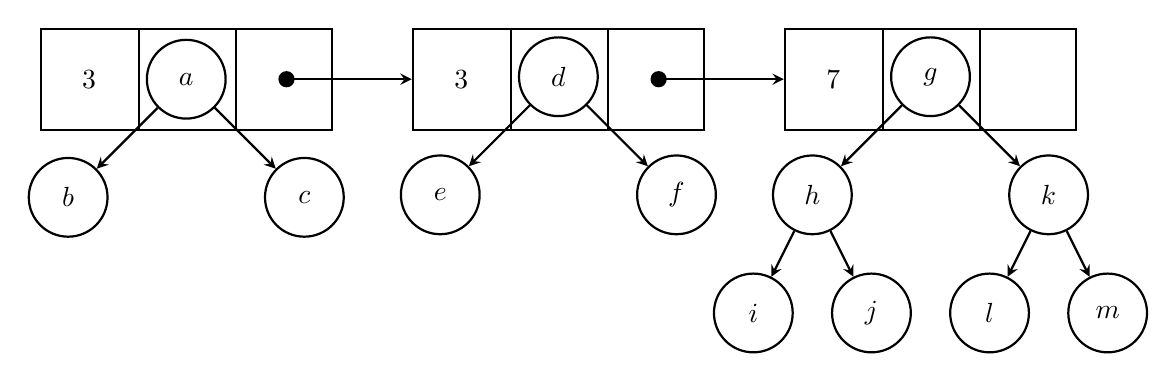
\begin{tikzpicture}[level distance=1.5cm,
  level 1/.style={sibling distance=3cm},
  level 2/.style={sibling distance=1.5cm},
  thick,->,auto,
  list/.style={rectangle split, rectangle split parts=3,
    draw, rectangle split horizontal,minimum size=15pt,inner sep=15pt}, >=stealth, start chain,
    desc/.style = {font=\tt, anchor=base, inner sep=2cm}]
    \tikzstyle{node}=[circle, minimum size=1cm, draw]
    
    \node[list,on chain]    	  (1st) {$3$};
    \node[node]         (a) {$a$}
      child{node[node]    (b) {$b$}}
      child{node[node]    (c) {$c$}};
      
    \node[list,on chain]    	  (2nd) {$3$};
    \node[node,below=-1.2cm of 2nd]         (d) {$d$}
      child{node[node]    (e) {$e$}}
      child{node[node]    (f) {$f$}};

    \node[list,on chain]    	  (3rd) {$7$};
    \node[node,below=-1.2cm of 3rd]         (d) {$g$}
     child{node[node]      (2) {$h$}
      child{node[node]    (4) {$i$}}
      child{node[node]    (5) {$j$}}}
    child{node[node]      (3) {$k$}
      child{node[node]    (6) {$l$}}
      child{node[node]    (7) {$m$}}};

  \draw[*->] let \p1 = (1st.three), \p2 = (1st.center) in (\x1,\y2) -- (2nd);
  \draw[*->] let \p1 = (2nd.three), \p2 = (2nd.center) in (\x1,\y2) -- (3rd);

  \end{tikzpicture}
\captionof{figure}{A list consisting of three complete binary trees, two of size 3 and one of size 7. An added node would result in two complete binary trees of size 7 and an additional node would result in one tree of size 15.}
\label{fig:two_lists_before_reverse}
\end{center}

Inserting new elements can at most join two trees. Since the left child of the resulting tree will be the first tree in the list and the right child will be the second tree, the tree can be constructed in constant time. Similarly, it can be destructed into two parts by just removing the root and cons the right child followed by the left child onto the list.

Looking up and element by index can be done by simply iterating the list until the containing tree has been found. If the index to search for is smaller than the size of the tree at the current position said tree will contain the element, otherwise subtract the size from the index and continue searching.

If we only have on complete binary tree looking up an element can clearly be done in $\BigO{\log n}$ time so we have to show that the length of the list will never be longer than $\log n$.

An integer on the form $2^k-1$ is called a skew-binary term, and if $t$ is such a term then the next skew-binary term will be $2t+1$. A decomposition of an integer $n$ greater or equal to zero will be a multiset of skew-binary terms $\{t_1,t_2,\cdots,t_m\}$ where $n = t_1 + t_2 + \cdots + t_m$. Such a decomposition is said to be greedy if the largest term is as large as possible and the remaining part of the decomposition is greedy as well. In other words a collection of skew-binary terms is greedy if no subset of lesser terms sums to a larger term. We will describe such a greedy decomposition of $n$ as $G(n)$.

\begin{prop}
\label{prop1}
Every integer $n \geq 0$ has a unique greedy decomposition.
\end{prop}
\begin{proof}
$G(0)$ will have the empty set which is unique. For $G(n)$ where $n>0$, we know, that no subset of skew-binary terms may sum to a larger term thus the it must include the largest possible term $t$ such that $t \leq n$. We add $t$ to the set and continue searching for $G(n-t)$.
Notice, that no subset of $G(n-t)$ can sum to $t$ otherwise it would not be the largest term respecting $t \leq n$.  
\end{proof}

\begin{prop} A skew-binary decomposition is greedy iif every term is unique except \label{prop2}
the two smallest: $t_1 \leq t_2 < t_3 < \cdots < t_m$.
\end{prop}
\begin{proof}
$\\ \Rightarrow$ We have a greedy decomposition and say we have two terms of size $2^k-1$ and a third term of equal or lesser size. Then the three terms would be greater or equal to another term because the next term would be at least as large as $2(2^k-1)+1$. But then this would not be greedy and we have a contradiction.\\
$\Leftarrow$ Again, because the next skew-binary term for any term $t$ is on the form $2t+1$, no two terms can sum up to another term if we only repeat the smallest ones twice and all others are unique. The decomposition would therefore be greedy.
\end{proof}

\begin{theorem} $|G(n)| \leq \lceil \log (n+1) \rceil$.
\label{thm1}
\end{theorem}
\begin{proof}
Clearly if $n=0$ it holds so we turn our attention to $n > 0$. Assume, to obtain a contradiction, that $|G(n)|$ contains more than $k=\lceil \log (n+1) \rceil$. Then, by \ref{prop2} and by how a greedy decomposition is defined, it must be that $G(n)$ contains a term at least as large as $2^k-1 \geq n$. Then, because $|G(n)|$ contains more than $k$ terms there is at least one more term and therefore the sum of terms in $G(n)$ will strictly exceed $n$ and we obtain a contradiction.
\end{proof}

Except for the two first trees in our list every size of the complete binary trees in the list is unique and in increasing order by construction. Therefore, the length of the list can not exceed $\lceil \log (n+1) \rceil$ by \ref{thm1}. Therefore, lookup will traverse at most $\BigO{\log n}$ elements in the list and perform a search in a single complete binary tree of height at most $\log n$.

\chapter{Conclusion}

\end{document}
